\documentclass{article}

\usepackage[load-configurations = abbreviations]{siunitx}
\usepackage{graphicx}
\usepackage{amsmath}
\usepackage{bm,upgreek}

\title{Analysis of Coupled Oscillators through Fourier Methods}
\author{Raymond Langehennig}

\begin{document}
\maketitle

\begin{abstract}
    test
\end{abstract}

\section{Introduction}

\subsection{Coupled and driven oscillators}
When a system exhibiting oscillatory motion (an oscillator) is subjected to a periodic, external force, it is known as a \emph{driven oscillator}. Driven oscillators exhibit a behavior known as \emph{resonance} when the frequency of the external force matches the oscillatory frequency of the system, at which point the amplitude of oscillation may increase dramatically, depending on how damped the system is.

A \emph{coupled oscillator} is a system with multiple oscillatory elements that influence each other in some way. This could be something like two pendulums connected by a spring, or the atoms of a metal connected by electromagnetism. For such a system, an arbitrary displacement from equilibrium usually results in complicated motion where the frequency at which each element oscillates itself continuously oscillates; however, coupled oscillators are capable of certain so-called \emph{normal modes} of motion, where each element oscillates at the same, fixed frequency. The number of different normal modes is equal to the number of degrees of freedom. This can be seen in the example of the two spring-coupled pendulums, for which there are two normal modes: the first when the two pendulums are given the same initial displacement in the same direction, and the second when they are given the same displacement but in opposite directions. When a coupled oscillator is driven, resonance may be achieved at the frequency of any one of these normal modes.

\subsection{Objective}
The subject of study in this report is a magnetically coupled, magnetically driven, torsional oscillator, and the object is to observe and analyze its motion with an oscilloscope and ultimately a fast Fourier transform spectrum analyzer, in order to find the frequencies of the normal modes.

\begin{figure}
    \centering
    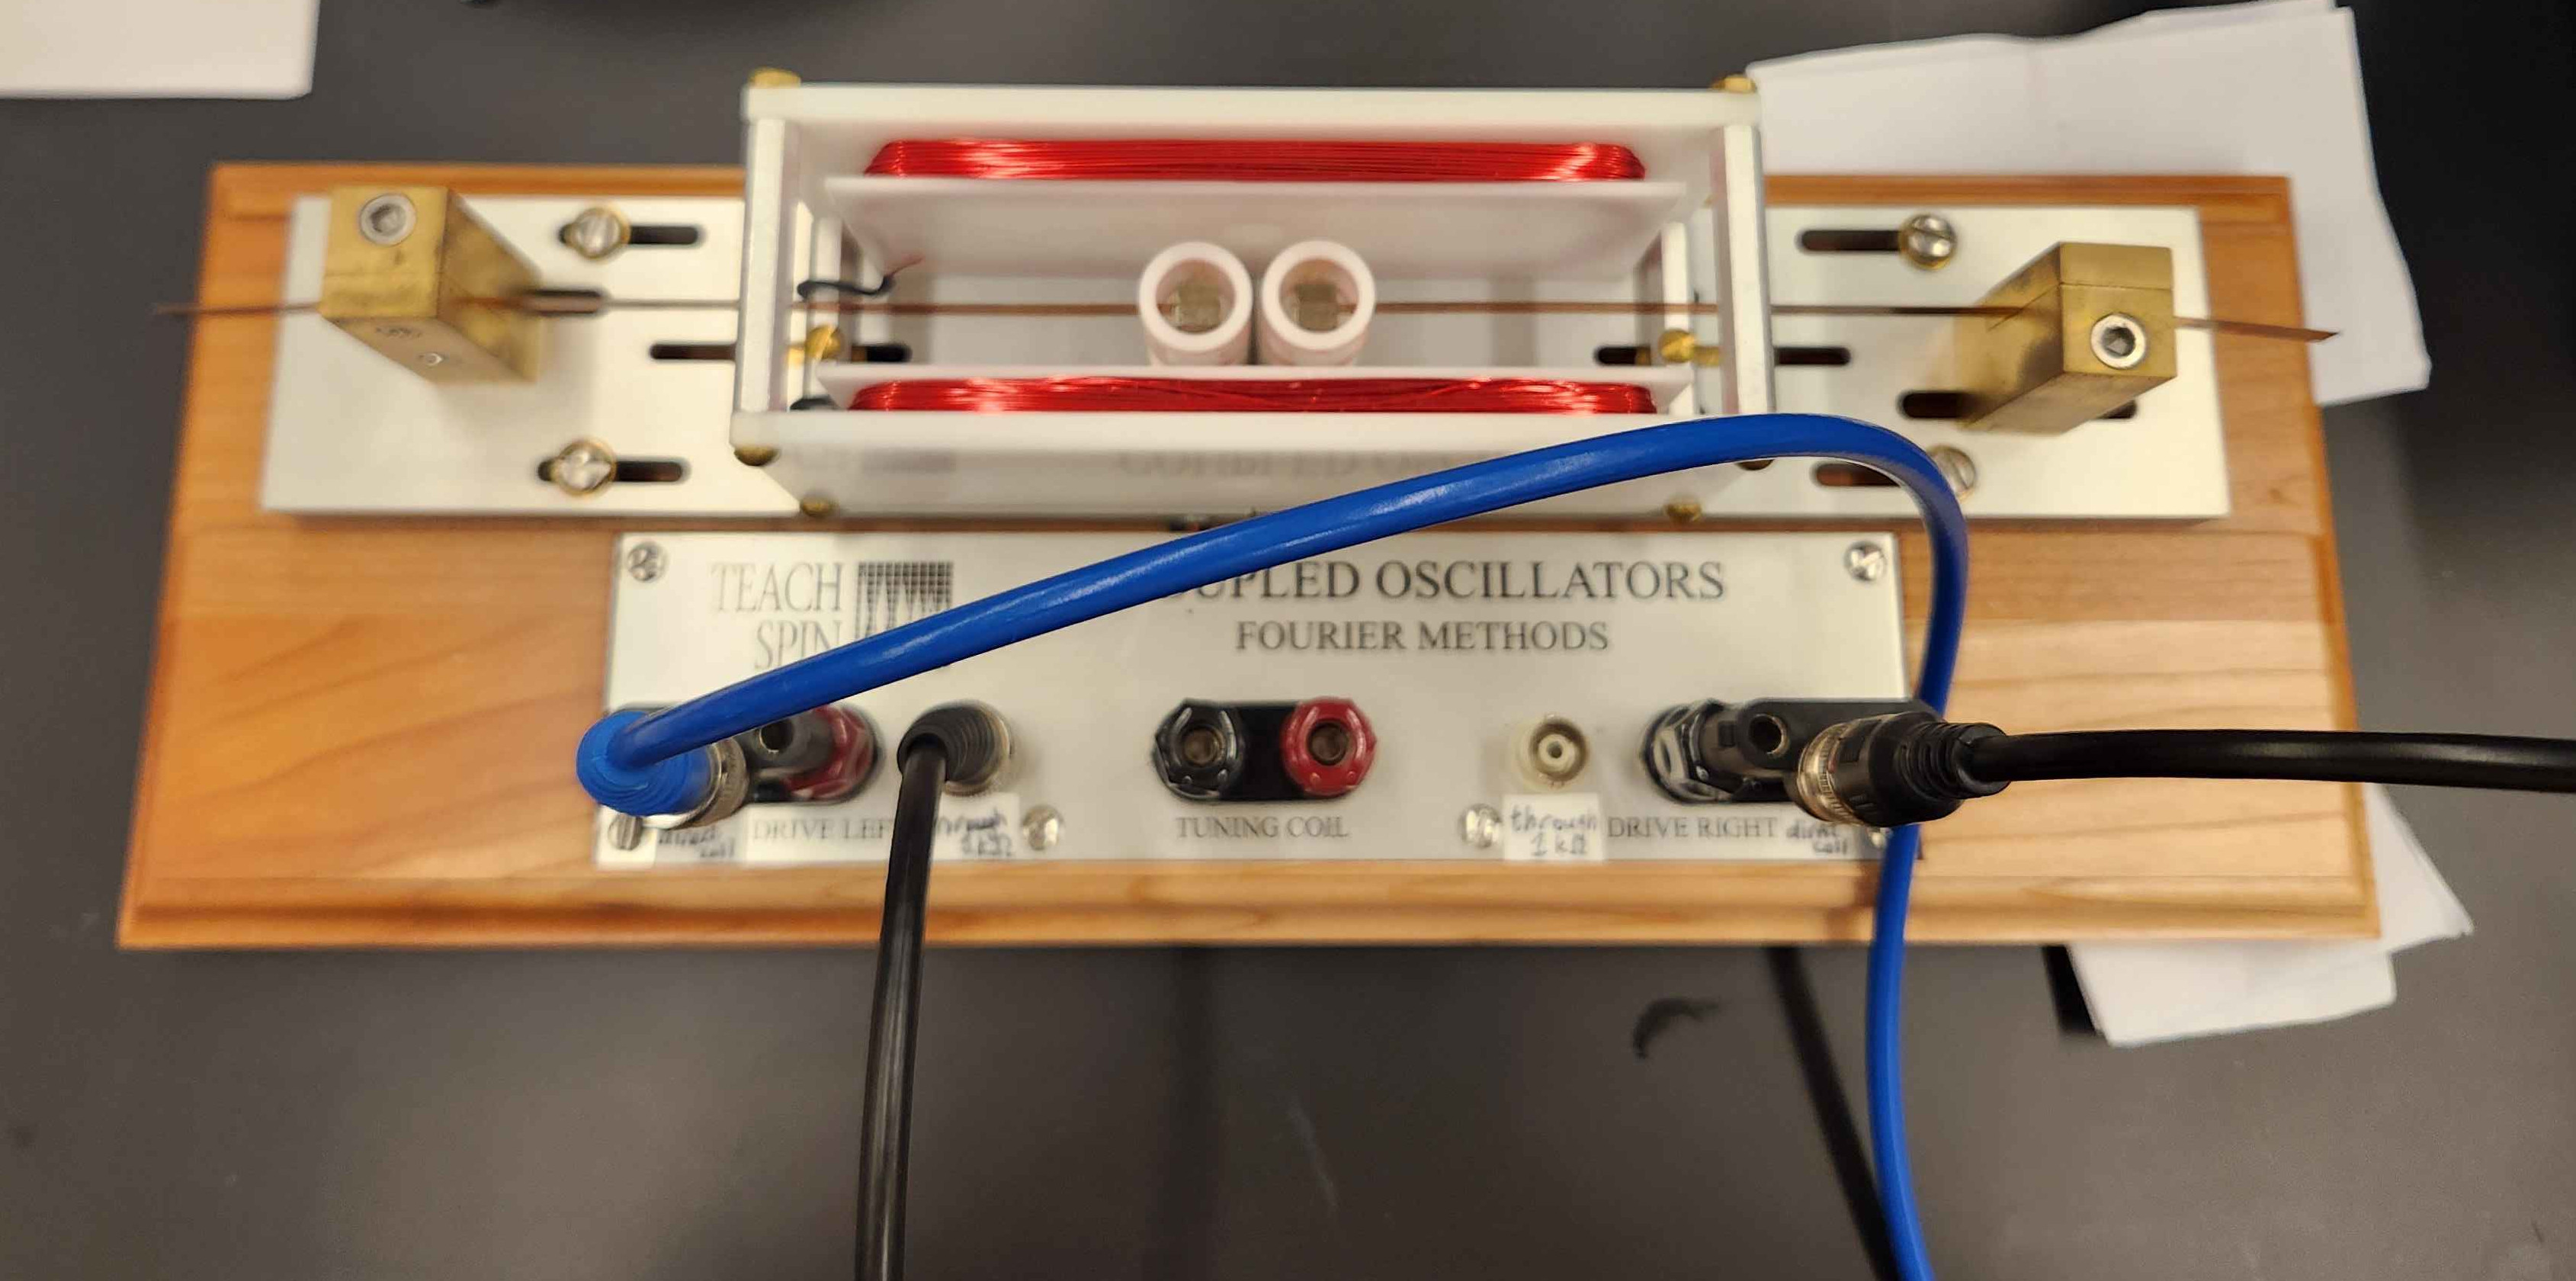
\includegraphics[width=0.5\linewidth]{20250910_113924.jpg}
    \caption{Photo of the torsional oscillator used.}
\end{figure}

\section{Model}
The oscillator consists of two phosphor-bronze reeds in-line with each other, clamped on the outer ends and with a magnetic neodymium cube either inner end. These magnets are placed inside vertical coils that allow for either excitation or detection, and both reeds are placed inside horizontal coils meant for tuning the entire system.
This setup means that there are two normal modes of oscillation, one where the reeds twist in phase and one where they twist completely out of phase. The frequencies of these normal modes may be predicted theoretically, after which they will be compared to experimental values.


\subsection{Resonsant frequency of a single reed}
The resonant frequency of a single, untuned reed can be calculated easily by $\omega = \sqrt{\kappa/I}$. $\kappa$ may be calculated using \[ \kappa = G\frac{wt^3}{3L}, \] where $G = \qty{41}{\giga\pascal}$ is the shear modulus, $w = \qty{6.35}{\mm}$ is the width of the reed, $t = \qty{0.254}{\mm}$ is the thickness or depth of the reed, and $L = \qty{100}{\mm}$ is the length of the reed, all giving $\kappa \approx \qty{0.014}{N.m}$. The rotational inertia of the cube $I = \rho\ell^5/6 \approx \qty{0.129}{\gram.\cm^2}$, with a density $\rho = \qty{7.51}{g/cm^3}$ and side length $\ell = \qty{6.35}{mm}$. This gives $\omega = \qty{1050}{\per\s}$ and therefore a resonant frequency $f = \qty{167}{Hz}$.

This is also one of the two resonant frequencies of the entire two-reed system (with no tuning), as will be shown in the derivation of the second resonant frequency, but which may also be seen from inspection.

\subsection{Resonant frequencies of the entire system}
Finding the resonant frequency of the second normal mode is a lot more involved. It entails finding the total potential energy of the entire system, with contributions from the torsion of the reeds, the tuning coils, and the interaction between the magnets, finding and finally solving the equations of motion of the system for the resonant frequencies.
\subsubsection{Tuning}
The tuning coils induce a magnetic field perpendicular to the axis of the reeds---in other words, if a coordinate system is given where $x$ is parallel to the reeds, $z$ is perpendicular to the ground, and $y$ is perpendicular to $x$ and $z$, the tuning field $B_T$ is in the $y$ direction. The tuning field effectively changes the torsion constant by adding a term to the potential energy
\begin{equation*}
    \begin{aligned}
        U   &= U_\tau + U_T \\
            &= \kappa\theta^2/2 - \bm{\upmu}\cdot\mathbf{B}_T \\
            &= \kappa\theta^2/2 - \mu B_T \cos \theta \\
            &\approx \kappa\theta^2/2 - \mu B_T (1-\theta^2/2) \\
            &= (\kappa+\mu B_T)\theta^2/2 - \mu B_T,
    \end{aligned}
\end{equation*}
where $\bm{\upmu}$ is the magnet's dipole. The new angular frequency can then be derived:
\begin{equation*}
    \begin{aligned}
        I \ddot{\theta} &= \tau = -\frac{\mathrm{d}U}{\mathrm{d}\theta} \\
            &= -(\kappa + \mu B_T)\theta \\
            &= -\omega^2 \theta \\
           \implies \omega &=  \sqrt{\frac{\kappa + \mu B_T}{I}}.
    \end{aligned}
\end{equation*}
If both reeds are considered, then they have two different frequencies,
\begin{equation*}
    \omega_1 = \sqrt{\frac{\kappa_1 + \mu_1 B_T}{I}}\quad\text{and}\quad\omega_2 = \sqrt{\frac{\kappa_2 - \mu_2 B_T}{I}},
\end{equation*}
where it is assumed the reeds have different torsional constants and dipole moments, and the negative in the second is because its magnet's moment is opposite that of the first.

\subsubsection{Coupling}
The interaction between the magnets may be modelled by considering the magnetic field at one of the two magnets due to the other, separated by a distance $\mathbf{r}$:
\begin{equation*}
    \mathbf{B}_1(\mathbf{r}) = \frac{\mu_0}{4\pi}\left( 3\frac{\bm{\upmu}_1\cdot\mathbf{r}}{r^5}\mathbf{r} - \frac{\bm{\upmu}_1}{r^3} \right),
\end{equation*}
from which arises a magnetic potential energy
\begin{equation*}
    \begin{aligned}
        U_B &= -\bm{\upmu}_2\cdot \mathbf{B}_1(\mathbf{r}) \\
            &= \frac{\mu_0}{4\pi}\left( -3\frac{(\bm{\upmu}_1\cdot\mathbf{r})(\bm{\upmu}_2\cdot\mathbf{r})}{r^5}\mathbf{r} + \frac{\bm{\upmu}_1\cdot\bm{\upmu}_2}{r^3} \right) \\
            &= \frac{\mu_0}{4\pi}\frac{\bm{\upmu}_1\cdot\bm{\upmu}_2}{r^3} \\
            &= -\frac{\mu_0}{4\pi}\frac{\mu_1\mu_2}{r^3}\cos(\theta_1 - \theta_2) \\
            &\approx -\frac{\mu_0}{4\pi}\frac{\mu_1\mu_2}{r^3} \left( 1 - \frac{(\theta_1 - \theta_2)^2}{2} \right)
    \end{aligned}
\end{equation*}
where the $\bm{\upmu}\cdot \mathbf{r}$ terms have gone to 0 as the two vectors are always perpendicular, and the small angle approximation has been applied to the cosine.

\subsubsection{Equations of motion}
The equation for the total potential energy, using the results of the previous sections, can be written
\begin{equation*}
    U = \frac{1}{2}\kappa\theta_1^2 + \frac{1}{2}\kappa\theta_2^2+ \frac{1}{2}\mu B_T\theta_1^2 + \frac{1}{2}\left( -\mu B_T \right)\theta_2^2 + \frac{1}{2}\left( -\frac{\mu_0}{4\pi}\frac{\mu^2}{r^3} \right)\left( \theta_1 - \theta_2 \right)^2,
\end{equation*}
where constant terms have been omitted (so that $U=0$ at some point) and the dipole moments and torsion spring constants are assumed to be equal in magnitude.
The coefficient in the last term, $-\frac{\mu_0}{4\pi}\frac{\mu^2}{r^3} := \lambda$, describes the strength of the magnetic coupling and comes out to about \qty{0.0008}{N.m} in magnitude for an $r$ of \qty{20}{mm}.

The equations of motion can now be derived:
\begin{equation*}
    \begin{cases}
        I\ddot{\theta}_1 &= -\frac{\partial U}{\partial \theta_1} + \mu k_z i_1 \\
        I\ddot{\theta}_2 &= -\frac{\partial U}{\partial \theta_2} + \mu k_z i_2
    \end{cases}
\end{equation*}
where $i_1$ and $i_2$ are the currents through the driving coils, and $k_z \approx \qty{6.6}{mT/A}$ gives the driving field strength generated by a current. These equations can be rewritten as
\begin{equation*}
    \begin{cases}
        I\ddot{\theta}_1 + (\kappa + \mu B_T)\theta_1 + \lambda(\theta_1 - \theta_2) &= \mu k_z i_1\\
        I\ddot{\theta}_2 + (\kappa - \mu B_T)\theta_2 + \lambda(\theta_2 - \theta_1) &= \mu k_z i_2
    \end{cases}
\end{equation*}
which are seen to be coupled differential equations.

This system of equations may be simplified by assuming the conditions the normal mode in the undriven case, where both currents are set to 0 and the system oscillates at $\omega$:
\begin{equation*}
    \begin{cases}
        \theta_1(t) &= A_1 \exp(-i\omega t) \\
        \theta_2(t) &= A_2 \exp(-i\omega t)
    \end{cases}
\end{equation*}
The coupled differential equations, now a linear system of equations, may be written in matrix form:
\begin{equation*}
    \left[ \begin{matrix}
        -I\omega^2+(\kappa + \mu B_T + \lambda)   &   -\lambda \\
        -\lambda                                    &   -I\omega^2+(\kappa - \mu B_T + \lambda)
    \end{matrix} \right]\left[ \begin{matrix} A_1 \\ A_2 \end{matrix} \right] = \left[ \begin{matrix} 0\\0 \end{matrix} \right].
\end{equation*}
For this equality to hold, either there is only the trivial solution where $A_1=A_2=0$, or there exists a nontrivial solution. The latter is true if and only if the determinant of the square matrix is 0.
This nontrivial case may be assumed by the fact the system exhibits oscillation,
\begin{equation*}
    \begin{aligned}
        \left| \begin{matrix}
        -I\omega^2+(\kappa + \mu B_T + \lambda)   &   -\lambda \\
        -\lambda                                    &   -I\omega^2+(\kappa - \mu B_T + \lambda)
    \end{matrix} \right| &= 0 \\
    = I^2 \omega^4 + \left(-2I\kappa-2I\lambda \right)\omega^2 + \left(\kappa^2 + 2\kappa\lambda - (\mu B_T)^2\right) &= 0,
    \end{aligned}
\end{equation*}
which is an easily solvable, biquadratic equation yielding
\begin{equation*}
    \omega = \sqrt{\frac{\kappa+\lambda \pm \sqrt{\lambda^2 + \left(\mu B_T\right)^2}}{I}},
\end{equation*}
where the negative solutions have been omitted.

\section{Materials and Procedure}


\section{Results}
\subsection{Raw data}
\subsection{Processed data}

\section{Conclusion}
ummmm damping



\end{document}
